% Created 2017-11-15 Wed 08:51
% Intended LaTeX compiler: pdflatex
\documentclass[a4paper,twoside,11pt]{article}
                              \usepackage[T1]{fontenc}
\usepackage{libertine}
\renewcommand*\oldstylenums[1]{{\fontfamily{fxlj}\selectfont #1}}
\usepackage{lmodern}
\usepackage[margin=1.0in]{geometry}
\usepackage{rotating}
\usepackage{setspace,amsmath,amsfonts,amssymb,bm}
\usepackage{graphicx}
\usepackage[usenames,dvipsnames]{xcolor}
\definecolor{Red}{rgb}{0.5,0,0}
\definecolor{NavyBlue}{rgb}{0.1,0.1,0.45}
\definecolor{MidnightBlue}{rgb}{0.1,0.1,0.65}
\usepackage[pdftex,hyperfootnotes=true,plainpages=false,pdfpagelabels,hypertexnames=true,naturalnames,pdfproducer={Latex},pdfcreator={pdflatex},bookmarks,bookmarksnumbered,colorlinks,linkcolor=MidnightBlue,citecolor=NavyBlue,filecolor=black,urlcolor=Red,breaklinks=true]{hyperref}
\usepackage{authblk}
\usepackage{xspace,helvet}
\usepackage{moreverb}
\usepackage{url, booktabs}
\usepackage{cleveref}
\usepackage[pdftex]{lscape}
\usepackage{fullpage}
\usepackage{booktabs}
\usepackage{multirow}
\usepackage{rotating}
\usepackage{pifont}
\usepackage{setspace}
\usepackage{threeparttable}
\usepackage{tabulary}
\usepackage[toc,page]{appendix}
\usepackage{pbox}
\usepackage[font=small]{caption}
\newcommand{\rom}[1]{\uppercase\expandafter{\romannumeral #1\relax}}
\newcommand{\E}{\mathsf{E}}
\newcommand{\VAR}{\mathsf{VAR}}
\newcommand{\COV}{\mathsf{COV}}
\newcommand{\Prob}{\mathsf{P}}
\newcommand{\RNum}[1]{\uppercase\expandafter{\romannumeral #1\relax}}
\newcommand{\dee}{\,\mbox{d}}
\newcommand{\naive}{na\"{\i}ve }
\newcommand{\eg}{e.g.\xspace}
\newcommand{\ie}{i.e.\xspace}
\newcommand{\pdf}{pdf.\xspace}
\newcommand{\etc}{etc.\@\xspace}
\newcommand{\PhD}{Ph.D.\xspace}
\newcommand{\MSc}{M.Sc.\xspace}
\newcommand{\BA}{B.A.\xspace}
\newcommand{\R}{\texttt{R}\xspace}
\usepackage{paralist}
\let\itemize\compactitem
\let\description\compactdesc
\let\enumerate\compactenum
\let\enumerate\inparaenum
\renewenvironment{enumerate}{\begin{inparaenum}[(i)]}{\end{inparaenum}}
\renewenvironment{enumerate}{\begin{inparaenum}[(a)]}{\end{inparaenum}}
\usepackage[round]{natbib}
\author[1]{Tarak Kharrat}
\author[2]{Georgi N. Boshnakov}
\affil[1]{Salford Business School, University of Salford, UK.}
\affil[2]{School of Mathematics, University of Manchester, UK.}
\newcommand{\code}{\texttt}
\newcommand{\CountrDist}[1]{\texttt{"#1"}}
\date{\today}
\title{Fertility Data\\\medskip
\large Extensive Analysis}
\hypersetup{
 pdfauthor={},
 pdftitle={Fertility Data},
 pdfkeywords={},
 pdfsubject={},
 pdfcreator={Emacs 25.2.1 (Org mode 9.1.2)}, 
 pdflang={English}}
\begin{document}

\maketitle
\begin{abstract}
This document analyses in details the fertility data first discussed by
\citet{winkelmann1995duration} and further analysed by \citet{mcshane2008count}
and recently by \citet{baker2017event}.  The computation described in this
document is done in \texttt{R} \citep{Rcore} using the contributed package \texttt{Countr}
\citep{RpackageCountr}. The package implements the algorithms described in
\citet{baker2017event} and an improved version of the methods derived in
\citet{mcshane2008count} for the weibull-count models. For this example, we
compare the weibull-count model to the standard Poisson \texttt{glm} and describe
methods to select the best model and access the goodness of fit of the selected
model.
\end{abstract}


\section{Prerequisites}
\label{sec:org6fc46dd}

We will do the analysis of the data with package \texttt{Countr}, so we load it:
\begin{verbatim}
library(Countr)
\end{verbatim}

Packages \texttt{dplyr} \citep{dplyr2016} and \citep{xtable2016} provide usefull facilities
for data manipulation and presentation:
\begin{verbatim}
library(dplyr) 
library(xtable)
\end{verbatim}



\section{Data}
\label{sec:org94417ff}

The fertility dataset was first analysed by \citet{winkelmann1995duration} and
we are thankful to Blake McShane for sharing it with us. 
We changed somewhat the
format of the columns by replacing dummy variables with factor variables and
renaming them. For example, the dummy variables for the different religions are
replaced by a single variable \texttt{"Religion"}, a factor with levels Other,
Catholic, Muslim and Protestant. 
These reformatted data are shipped with package \texttt{Countr} and can
be loaded in the usual way:
\begin{verbatim}
data(fertility)
\end{verbatim}

% latex table generated in R 3.4.1 by xtable 1.8-2 package
% Mon Oct 23 17:26:22 2017
\begin{table}[ht]
\centering
\begin{tabular}{rrlrlllrlr}
  \hline
 & \begin{sideways} children \end{sideways} & \begin{sideways} german \end{sideways} & \begin{sideways} years\_school \end{sideways} & \begin{sideways} voc\_train \end{sideways} & \begin{sideways} university \end{sideways} & \begin{sideways} Religion \end{sideways} & \begin{sideways} year\_birth \end{sideways} & \begin{sideways} rural \end{sideways} & \begin{sideways} age\_marriage \end{sideways} \\ 
  \hline
1 &   2 & no &   8 & no & no & Other &  42 & yes &  20 \\ 
  2 &   3 & no &   8 & no & no & Other &  55 & yes &  21 \\ 
  3 &   2 & no &   8 & no & no & Other &  51 & yes &  24 \\ 
  4 &   4 & no &   8 & no & no & Other &  54 & no &  26 \\ 
  5 &   2 & no &   8 & no & no & Other &  46 & yes &  22 \\ 
  6 &   2 & no &   8 & no & no & Other &  41 & no &  18 \\ 
   \hline
\end{tabular}
\caption{First few rows of fertility data.} 
\label{tbl:data}
\end{table}

The first few rows of the data are shown in Table \ref{tbl:data}.
The sample is formed by observation of 
1243
women aged 44 or older in 1985 who answered the
questions relevant to the analysis conducted by the \emph{German Socio-Economic
Panel}. The count variable \texttt{children} is the number of births per woman and is
characterised by small \emph{underdispersion}: the variance of the number of births
is less than the mean, 
2.33
versus 
2.384

% latex table generated in R 3.4.1 by xtable 1.8-2 package
% Mon Oct 23 17:26:24 2017
\begin{table}[ht]
\centering
\begin{tabular}{rllllllllll}
  \hline
 & 0 & 1 & 2 & 3 & 4 & 5 & 6 & 7 & 8 & $>$= 9 \\ 
  \hline
Frequency & 76 & 239 & 483 & 228 & 118 & 44 & 30 & 10 & 8 & 7 \\ 
  Relative frequency & 0.061 & 0.19 & 0.39 & 0.18 & 0.095 & 0.035 & 0.024 & 0.008 & 0.0064 & 0.0056 \\ 
   \hline
\end{tabular}
\caption{Fertility data: Frequency distribution of column \texttt{children}.} 
\label{tbl:freq}
\end{table}

There are 
8
possible explanatory variables: 
3
continuous and 
5
categorical (factors), describing the risk of a birth, see the package documentation for
further details. 

This computes separate summaries for the numeric and non-numeric variables:
\begin{verbatim}
nam_fac <- sapply(fertility, function(x) !is.numeric(x))
fert_factor <- summary(fertility[ , nam_fac])
fert_num <- t(sapply(fertility[ , !nam_fac], summary))
\end{verbatim}

The results are shown in Tables \ref{tbl:frecfac} and \ref{tbl:frecnum}.
% latex table generated in R 3.4.1 by xtable 1.8-2 package
% Mon Oct 23 17:26:25 2017
\begin{table}[ht]
\centering
\begin{tabular}{rlllll}
  \hline
 & german & voc\_train & university &       Religion & rural \\ 
  \hline
1 & no :245   & no :704   & no :1207   & Other     :130   & no :613   \\ 
  2 & yes:998   & yes:539   & yes:  36   & Catholic  :502   & yes:630   \\ 
  3 &  &  &  & Muslim    : 75   &  \\ 
  4 &  &  &  & Protestant:536   &  \\ 
   \hline
\end{tabular}
\caption{Summary of the factor variables} 
\label{tbl:frecfac}
\end{table}


% latex table generated in R 3.4.1 by xtable 1.8-2 package
% Wed Nov 15 08:49:57 2017
\begin{table}[ht]
\centering
\begin{tabular}{rrrrrrr}
  \hline
 & Min. & 1st Qu. & Median & Mean & 3rd Qu. & Max. \\ 
  \hline
children & 0.00 & 1.00 & 2.00 & 2.38 & 3.00 & 11.00 \\ 
  years\_school & 8.00 & 9.00 & 9.00 & 9.10 & 9.00 & 13.00 \\ 
  year\_birth & 40.00 & 45.00 & 50.00 & 51.99 & 58.00 & 83.00 \\ 
  age\_marriage & 17.00 & 21.00 & 23.00 & 23.11 & 25.00 & 30.00 \\ 
   \hline
\end{tabular}
\caption{Summary of the numeric explanatory variables} 
\label{tbl:frecnum}
\end{table}




\section{Fitting a model}
\label{sec:org0f503d8}

The benchmark for this data set is the Poisson \texttt{glm}. It can be fitted in the
usual way using the \texttt{glm()} function.
\begin{verbatim}
form <- children ~ german + years_school + voc_train + university + Religion +
    year_birth + rural + age_marriage
pois <- glm(formula = form, data = fertility, family = poisson())
summary(pois)
\end{verbatim}

\phantomsection
\label{org06e8a44}
\begin{verbatim}

Call:
glm(formula = form, family = poisson(), data = fertility)

Deviance Residuals: 
    Min       1Q   Median       3Q      Max  
-3.1839  -0.6964  -0.0792   0.4088   4.1954  

Coefficients:
                    Estimate Std. Error z value Pr(>|z|)    
(Intercept)         1.147444   0.301658   3.804 0.000142 ***
germanyes          -0.200362   0.072135  -2.778 0.005476 ** 
years_school        0.033506   0.032455   1.032 0.301901    
voc_trainyes       -0.152776   0.043856  -3.484 0.000495 ***
universityyes      -0.154830   0.158779  -0.975 0.329498    
ReligionCatholic    0.218038   0.070716   3.083 0.002047 ** 
ReligionMuslim      0.547571   0.085039   6.439 1.20e-10 ***
ReligionProtestant  0.113410   0.076272   1.487 0.137038    
year_birth          0.002418   0.002383   1.015 0.310213    
ruralyes            0.059072   0.038120   1.550 0.121224    
age_marriage       -0.030446   0.006510  -4.677 2.91e-06 ***
---
Signif. codes:  0 '***' 0.001 '**' 0.01 '*' 0.05 '.' 0.1 ' ' 1

(Dispersion parameter for poisson family taken to be 1)

    Null deviance: 1204.3  on 1242  degrees of freedom
Residual deviance: 1034.4  on 1232  degrees of freedom
AIC: 4225.6

Number of Fisher Scoring iterations: 5
\end{verbatim}

One alternative to the standard Poisson model is the renewal count models
implemented in \texttt{Countr}. In theory, any survival density can be used to build
the associated renewal-count model using the computation methods detailed in
\citet{baker2017event}.


\subsection{Distributions}
\label{sec:orga269afd}

The package offers several choices for the inter-arrival times distribution.
The overview here is for \texttt{Countr} version 3.4.1.
There are three main distributions:
\code{weibull}, \code{gamma} and \code{gengamma} (generalised gamma). They
should work fine with all data sets. There are also some experimental
distributions, \code{weibullgam} 
\citep[weibull-gamma, see][Section 3.2]{mcshane2008count} and \code{burr}, 
which should be used with care. Users can also use their own \texttt{dist = "custom"}
distributions but the computation times in this case may become cumbersome and
should be avoided with large datasets.


\subsection{Algorithms}
\label{sec:org2b8bfc7}

Three main algorithms have been implemented to compute the associated
convolution problem in the function \texttt{renewalCount()} and can be specified by
choosing the desired method in the \texttt{convPars} argument. The performance of the
different algorithms has been compared in \citet[Section 7.2]{baker2017event}.
The default set-up is to use the \texttt{dePril} algorithm with 50 steps and
extrapolation. We found that this set-up worked quite well for a large range of
examples. The weibull-count model can also be fitted using 2 series expansion
methods. These algorithms are usually faster but less reliable for large counts
(>= 10).

The following code fits a weibull-count model to the \texttt{fertility} data using the
default algorithm and the \texttt{PORT} optimisation routine (\code{nlminb}).

\begin{verbatim}
form <- children ~ german + years_school + voc_train + university + Religion +
    year_birth + rural + age_marriage
wei <- renewalCount(formula = form, data = fertility, dist = "weibull",
                    weiMethod = "conv_dePril",
                    control = renewal.control(trace = 0, method = "nlminb")
                    )
summary(wei)
\end{verbatim}

\begin{verbatim}

Call:
renewalCount(formula = form, data = fertility, dist = "weibull", 
    control = renewal.control(trace = 0, method = "nlminb"), 
    weiMethod = "conv_dePril")

Pearson residuals:
    Min      1Q  Median      3Q     Max 
-2.6721 -0.9975 -0.2462  0.4292  7.1926 
Inter-arrival dist.: weibull 
              Links: scale: link log, shape: link log 

Count model coefficients
                          Estimate Std. Error z value Pr(>|z|)    
scale_                    1.397176   0.304994   4.581 4.63e-06 ***
scale_germanyes          -0.222547   0.072208  -3.082 0.002056 ** 
scale_years_school        0.038533   0.032604   1.182 0.237269    
scale_voc_trainyes       -0.173348   0.043996  -3.940 8.15e-05 ***
scale_universityyes      -0.181454   0.159394  -1.138 0.254953    
scale_ReligionCatholic    0.241996   0.070708   3.422 0.000621 ***
scale_ReligionMuslim      0.638743   0.086420   7.391 1.46e-13 ***
scale_ReligionProtestant  0.123141   0.076195   1.616 0.106064    
scale_year_birth          0.002305   0.002383   0.967 0.333439    
scale_ruralyes            0.068059   0.038169   1.783 0.074570 .  
scale_age_marriage       -0.034026   0.006537  -5.205 1.94e-07 ***
shape_                    0.211969   0.027268   7.773 7.64e-15 ***
---
Signif. codes:  0 '***' 0.001 '**' 0.01 '*' 0.05 '.' 0.1 ' ' 1 

Number of iterations in nlminb optimization: 48 

Execution time   39 
Log-likelihood: -2077.0244 on 12 Df
\end{verbatim}

Note that the scale (\texttt{scale\_}) and shape (\texttt{shape\_}) parameters are reported on
the log scale in this example and hence in order to recover the values in
\citep[Table 2]{mcshane2008count}, one should apply \texttt{exp()} to the coefficient
values.


\section{Residuals}
\label{sec:org7a154d6}

Residuals measure the departure of fitted values from observed values of
the response variables. 
They can be used to detect model misspecification:
outliers, poor fit for given values of the covariates and/or the count
values. Whereas a universal definition of residuals exists for linear models (the
difference, possibly standardised, between observed and fitted values), 
this universality is lost for
nonlinear models. Many definitions have been suggested in the literature (see
the discussion in \citet[Section 5.2]{cameron2013regression}) and depending on the
aims of the analysis, one definition may be more useful than another.

For renewal-count models, the Pearson residuals are easy to compute and can be
used in diagnostoc plots. Such plots need to be interpreted with care however
since there are no theoretical results for renewal-count models justifying the
asymptotic normality of residuals. There is also little hope to make them
identically distributed.

The \texttt{Countr} package provides a method to compute Peason residuals and a routine
\texttt{residuals\_plot()} to plot them in order to assist the analyst when trying to
work out some patterns that would lead to model improvement (detect outliers,
introduce covariates in a different form, etc.).

\begin{verbatim}
residuals_plot(wei, type = "pearson")
\end{verbatim}


\begin{figure}[htbp]
\centering
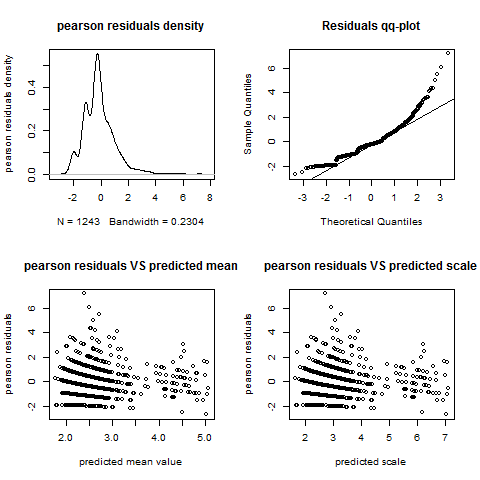
\includegraphics[width=.9\linewidth]{wei_residuals.png}
\caption{\label{fig:org56d5660}
Weibull model: residuals analysis}
\end{figure}

In Figure \ref{fig:org56d5660}, four diagnosis plots are presented for the
fitted weibull count model. The top left graph shows the estimated density of
the residuals. The distribution has a mode around zero, is slightly right skewed
and has fat tails. The departure from normality is confirmed in the qq-plot
(top-right) especially for large values of the residuals (absolute values larger
than 2). The bottom graphs plot the residuals against the predicted mean and
predicted scale and show the presence of some outliers.

One can also compare the residuals of the previously fitted models (Poisson and
Weibull):

\begin{verbatim}
par(mfrow = c(1, 2))
res_wei <- residuals(wei, type = "pearson")
qqnorm(res_wei, ylim = range(res_wei), main = "Weibull Renewal Model")
qqline(res_wei, ylim = range(res_wei))
grid()
pois <- glm(formula = form, data = fertility, family = poisson())
res_pois <- residuals(pois, type = "pearson")
qqnorm(res_pois, ylim = range(res_wei), main = "GLM Poisson")
qqline(res_pois, ylim = range(res_wei))
grid()
\end{verbatim}

\begin{figure}[htbp]
\centering
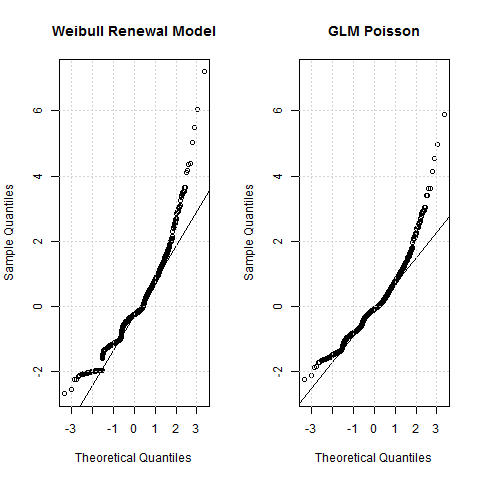
\includegraphics[width=.9\linewidth]{compare_residuals.png}
\caption{\label{fig:org4fef672}
Normal QQ-plots for the Weibull and Poisson Pearson's residuals. Both are clearly not normal.}
\end{figure}

Figure \ref{fig:org4fef672} shows that the Weibull and Poisson Pearson's
residuals are not normal. It could be speculated that the Poisson's residuals
are somewhat closer to normality but this is doesn't really give az basis for
informed decision.


\section{Statistical Tests}
\label{sec:org0ecd51a}

The Poisson and weibull models can be considered nested. In fact, the Poisson
model is a special case of the weibull with a shape parameter equal to 1 (0 on
the log scale).


\subsection{t-test}
\label{sec:org0719a27}

Based on the previous observation, one can test the significance of the shape
parameter using the usual \emph{t-test}. The \emph{t-test} is a special case of the Wald
test (see \citet[Section 2.6]{cameron2013regression}). Let \(\theta\) be the
regression coefficients and \(j\) be the index of the shape parameter. The
null hypothesis is defined as \(H_0: \ \theta_j = 0\) to be tested against the
alternative hypothesis  \(H_a: \ \theta_j \neq 0\). The test statistic \(T_z\) is defined by:
\begin{equation}
   T_z = \frac{\hat{\theta}_j}{\sqrt{v_{jj}}}
\end{equation}
where \(\hat{\theta}_j\) is the estimated shape parameter and \(\sqrt{v_{jj}}\) its
estimated standard error. Asymptotically, \(T_z\) is standard normal. We reject
\(H_0\) against \(H_a\) at significance level \(\alpha\) if \(|T_z| > z_{\alpha / 2}\).

Following standard practice in \texttt{R}, the \emph{t-test} and the associated p-values are
reported when calling the \texttt{summary()} method for a fitted regression
model. Therefore, in order to obtain the value of the \emph{t-test} for the shape
value, the user can use the following code:

\begin{verbatim}
form <- children ~ german + years_school + voc_train + university + Religion +
                   year_birth + rural + age_marriage
wei <- renewalCount(formula = form, data = fertility, dist = "weibull",
                    control = renewal.control(trace = 0, method = "nlminb")
                    )
wei_summary <- summary(wei)$coef
\end{verbatim}


\begin{verbatim}
t_shape <- wei_summary[rownames(wei_summary) == "shape_",, drop = FALSE]
print(xtable(t_shape), floating = FALSE)
\end{verbatim}

% latex table generated in R 3.4.1 by xtable 1.8-2 package
% Mon Oct 23 17:28:28 2017
\begin{tabular}{rrrrr}
  \hline
 & Estimate & Std. Error & z value & Pr($>$$|$z$|$) \\ 
  \hline
shape\_ & 0.21 & 0.03 & 7.79 & 0.00 \\ 
   \hline
\end{tabular}


The test statistic is
T\(_{\text{z}}\) = 7.794,
which means that \(H_0\) can be rejected at any reasonable significance
level. Therefore, according to the \emph{t-test}, the Poisson model can be rejected
in favour of the weibull one.


\subsection{Likelihood ratio test}
\label{sec:org3eb7809}

Given that the estimation procedure for both models is likelihood based, one
classical statistical technique for testing hypotheses (for nested models) is the
likelihood ratio test. One can formulate the null hypothesis as being in favour
of the Poisson model. The \emph{likelihood ratio test statistic} is defined as:
\begin{equation}
    T_{LR} = -2[L_0 - L_a]
 \end{equation}
which is assymptotically \(\chi^2(h)\) under \(H_0\) and \(h\) is the difference in
degree of freedom between the models (here \(h=1\)). \(H_0\) is rejected against
\(H_a\) at significance level \(\alpha\) if \(T_{LR} > \chi^2(h;\alpha)\).

In \texttt{R}, one can use the \texttt{lmtest} package \citep{lmtest2002} to conduct the
likelihood ratio test as shown below:

\begin{verbatim}
library(lmtest)
lrtest(pois, wei)
\end{verbatim}

\begin{verbatim}
[1] "7.794"
Likelihood ratio test

Model 1: children ~ german + years_school + voc_train + university + Religion + 
    year_birth + rural + age_marriage
Model 2: children ~ german + years_school + voc_train + university + Religion + 
    year_birth + rural + age_marriage
  #Df  LogLik Df  Chisq Pr(>Chisq)    
1  11 -2101.8                         
2  12 -2077.0  1 49.559  1.925e-12 ***
---
Signif. codes:  0 '***' 0.001 '**' 0.01 '*' 0.05 '.' 0.1 ' ' 1
Warning message:
In modelUpdate(objects[[i - 1]], objects[[i]]) :
  original model was of class "glm", updated model is of class "renewal"
\end{verbatim}

The \texttt{warning} message simply reminds the user that the models have different
classes and can be safely ignored here. The test shows that H\(_{\text{0}}\) can be rejected
at any significance level and comforts the conclusion of the \emph{t-test} described
earlier: The Weibull model should be preferred to the Poisson for the fertility
data.


\section{Goodness of Fit}
\label{sec:org3a46ca5}

For fully parametric models such as Poisson or renewal-count, a crude diagnosis
is to compare the fitted probabilities with observed frequencies. Things are
better understood with a formula. Define the count variable \(y_i, i=1, \dots, n\)
where \(n\) is the total number of individuals and let \(m = max(y_i)\). We denote
by \(\bar{p}_j\) the observed frequencies (the fraction of the sample where \(y =
j\)) and let \(\hat{p}_j, j = 1, \dots, m\) the fitted frequencies. For example, in
the Poisson model, \(\hat{p}_j = \frac{1}{n} \sum_{i=1}^{n} \exp{(-\hat{\mu}_i^j) /
j!}\).

To start with, one can compare \(\bar{p}_j\) to \(\hat{p}_j\) for specific values of
the count variable \(j\) to gain some insight about the range of counts where the
model has a tendency to over or under predicts or to allow a visual inspection
of the predictive performance of competing models. This computation can be done
in \texttt{Countr} by a call to the function \texttt{compareToGLM} which can take a fitted
Poisson and (optionally) a negative binomial model and compare them to a number
of fitted \texttt{renewal} models passed in \texttt{...}. The function will return a table
with \(\bar{p}_j\) (\texttt{Actual}) and the \(\hat{p}_j\) induced by the different
models. The contribution to the Pearson statistic of each cell defined as
\(\sum_{j=1}^J n\frac{(\bar{p}_j - \hat{p}_j)^2}{\bar{p}_j}\) will also be
computed. Note that here we specified the cells by providing the \texttt{breaks}
argument: the two cells 5-6 and 7-8 were merged and counts larger than 9 have
also been merged.

\begin{verbatim}
form <- children ~ german + years_school + voc_train + university + Religion +
    year_birth + rural + age_marriage
pois <- glm(formula = form, data = fertility, family = poisson())
wei <- renewalCount(formula = form, data = fertility, dist = "weibull",
                    control = renewal.control(trace = 0, method = "nlminb")
                    )
tab <- compareToGLM(poisson_model = pois, breaks = c(0:5, 7, 9), weibull = wei)
tab_tbl <- xtable(tab, caption = "Comparison between some models.")
print(tab_tbl)
\end{verbatim}

% latex table generated in R 3.4.1 by xtable 1.8-2 package
% Wed Nov 15 08:48:08 2017
\begin{table}[ht]
\centering
\begin{tabular}{rlrrrrr}
  \hline
 & Counts & Actual & weibull\_predicted & poisson\_predicted & weibull\_pearson & poisson\_pearson \\ 
  \hline
1 & 0 & 0.06 & 0.07 & 0.10 & 0.52 & 22.66 \\ 
  2 & 1 & 0.19 & 0.23 & 0.23 & 7.17 & 6.60 \\ 
  3 & 2 & 0.39 & 0.29 & 0.25 & 42.15 & 90.97 \\ 
  4 & 3 & 0.18 & 0.22 & 0.19 & 6.33 & 0.69 \\ 
  5 & 4 & 0.09 & 0.12 & 0.12 & 5.04 & 4.93 \\ 
  6 & 5-6 & 0.06 & 0.07 & 0.09 & 2.30 & 10.16 \\ 
  7 & 7-8 & 0.01 & 0.01 & 0.02 & 2.58 & 0.22 \\ 
  8 & $>$= 9 & 0.01 & 0.00 & 0.00 & 18.40 & 2.71 \\ 
   \hline
\end{tabular}
\caption{Comparison between some models.} 
\end{table}



In a first step, one can compare the Pearson statistics:
\begin{verbatim}
colSums(dplyr::select(tab, contains("_pearson")))
\end{verbatim}

\begin{verbatim}
weibull_pearson poisson_pearson 
       84.48827       138.94820
\end{verbatim}


It can be seen that the Pearson statistic for the Poisson model is 40\% larger
than the one achieved by the weibull model. It is also interesting to note the
contribution to the Pearson statistic is substantially smaller in the Poisson
case for cells 7-8 and 9 and larger. This was already observed in the residuals
plot and shows the Poisson model presents a 'better' fit in the tails and hence
is less robust to outliers. In fact, the Poisson fitting process focuses on
minimising the 'mean-error' and hence the estimation maybe influenced by
outliers (It is well known that the mean is not robust to outliers). The weibull
model with the extra shape parameter somehow smooths this effect. Depending on
the analyst goal (predicting the mean or the different probabilities), this
feature maybe seen as a desired addition. For more on this, see the discussion
in \citet[Section 6.2]{cameron2013regression}).

More insight can be gained by visualising the previous results. This can be done
by calling the function \texttt{frequency\_plot()} as follows:
\begin{verbatim}
frequency_plot(tab$Counts, tab$Actual,
               dplyr::select(tab, contains("_predicted"))
)
\end{verbatim}

\begin{center}
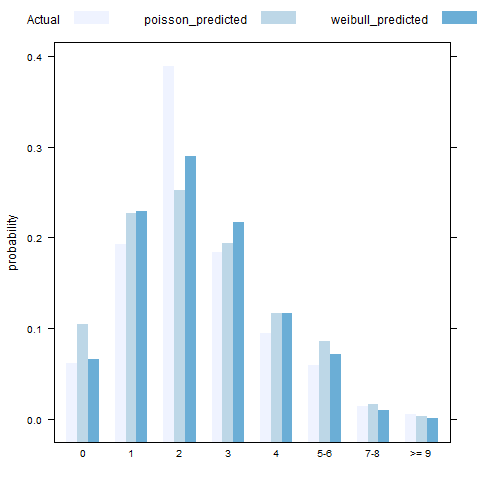
\includegraphics[width=.9\linewidth]{hist.png}
\end{center}



Visualising the result can be a good starting point but without a formal test,
it is hard to conclude if \(\hat{p}_j\) is a \emph{good approximation} to \(\bar{p}_j\)
and hence if the model fits the data well. \citet[Section 5.3.4]{cameron2013regression})
suggest a formal \emph{chi-square goodness-of-fit
test} which is a generalisation of the Pearson's \emph{chi-square test} and controls
for estimation error in \(\hat{p}_j\). The test is a conditional moment test. It
has been implemented in \texttt{Countr} in the \texttt{chiSq\_gof()} method using the gradient
version which is justified for renewal models as they are fully parametric and
parameters estimated is based on maximum-likelihood.

\begin{verbatim}
  form <- children ~ german + years_school + voc_train + university + Religion +
      year_birth + rural + age_marriage
  wei <- renewalCount(formula = form, data = fertility, dist = "weibull",
                      control = renewal.control(trace = 0, method = "nlminb")
                      )
  gof <- chiSq_gof(wei, breaks = c(0:5, 7, 9))
  gof
\end{verbatim}

\begin{verbatim}
chi-square goodness-of-fit test

Cells considered 0 1 2 3 4 5-6 7-8 >= 9
  DF  Chisq Pr(>Chisq)    
1  7 70.167  1.367e-12 ***
---
Signif. codes:  0 '***' 0.001 '**' 0.01 '*' 0.05 '.' 0.1 ' ' 1
\end{verbatim}

The formal chi-square test statistic yields a value 
70.17, compared to
\(\chi^{\text{2}}\)(7) critical value of 12.02 at 5\%. The weibull model, although preferred to
the Poisson according to the LR test, is strongly rejected. For this type of
models with bi-modal distribution, mixture models are usually preferred. See the
discussion in \citet[Chapter 6.2]{cameron2013regression}.
\section{Conclusion}
\label{sec:orge56249e}

The above analysis suggests, on several measures, that 
the weibull count model is better than the Posson model for the fertility
dataset but it may not be good enough, as well. 



\label{sec:orgebcc268}
\bibliographystyle{apalike}
\bibliography{REFERENCES}
\end{document}
